\section{ТЕСТИРОВАНИЕ И ВЕРИФИКАЦИЯ ЧИСЛЕННОЙ МОДЕЛИ}

В данном разделе представлены результаты тестирования разработанного численного алгоритма. Основное внимание уделено исследованию точности и производительности метода в зависимости от параметров дискретизации, а также сравнению полной и параболизированной постановок уравнений. Для сравнения точности были выбраны расчёты из~\cite{book11_tur}.

\subsection{Зависимость точности решения от шага дискретизации}

Сравнение проводилось для трёх случаев $H_1 = 0.0150, H_2 = 0.0075, H_3 = 0.0037$. Результаты проверялись по значениям переменной $U$. Входные данные сохранены в фалйе \texttt{test7.py} на GitHub репозитории проекта (ссылка в приложении).

Для анализа влияния шага дискретизации на точность решения была рассмотрена модельная задача о ламинарной струе с химическими реакциями. Исследование проводилось при различных значениях шага по пространству $\Delta x, \Delta y$ и времени $\Delta t$. Как видно из рисунках~\ref{fig:acc_1_1},~\ref{fig:acc_1_2},~\ref{fig:acc_2_1},~\ref{fig:acc_2_2},~\ref{fig:acc_3_1},~\ref{fig:acc_3_2}, уменьшение шага приводит к монотонному снижению погрешности до некоторого предельного значения. 

\begin{figure}
    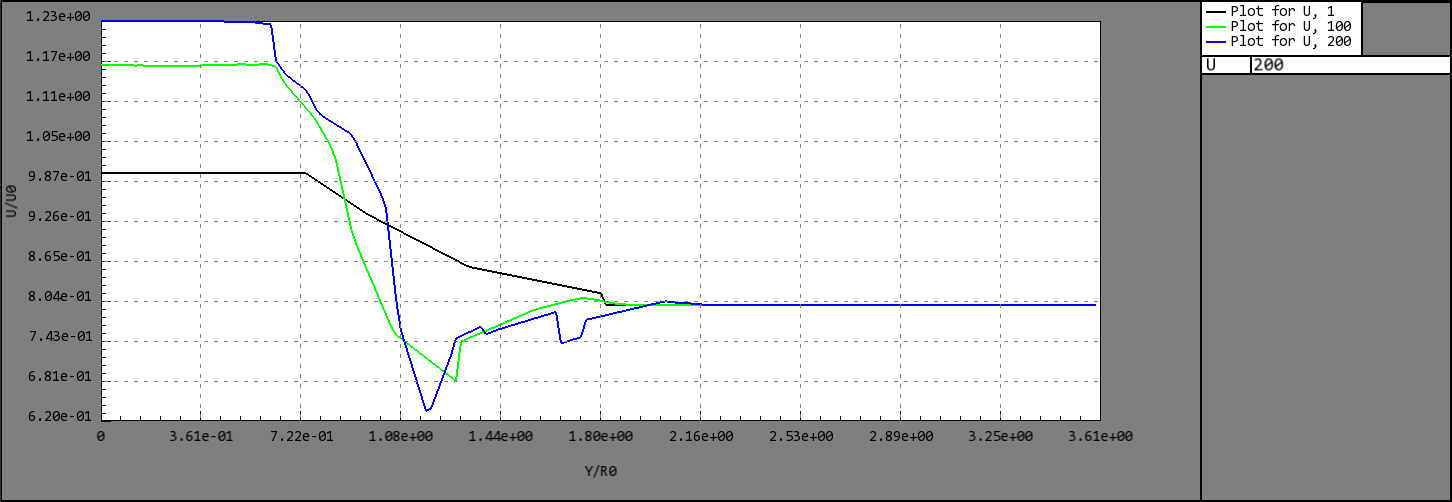
\includegraphics[width=15cm]{2-05-test1}
    \caption{Значение шага $0.015$, параболизованная система}
    \label{fig:acc_1_1}
\end{figure}

\begin{figure}
    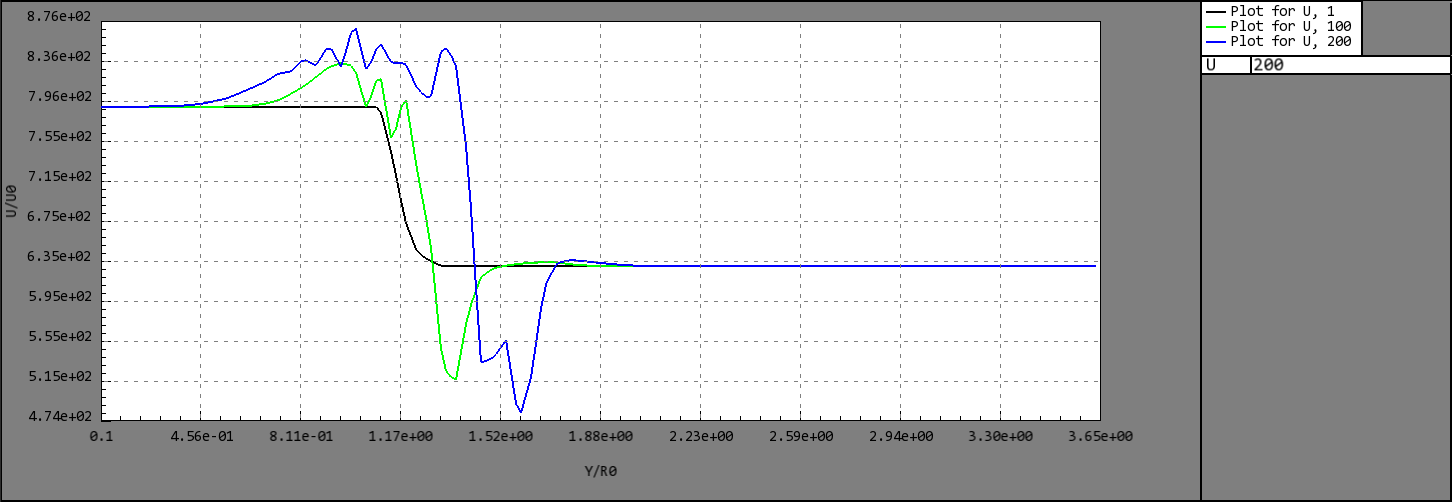
\includegraphics[width=15cm]{2-05-test4}
    \caption{Значение шага $0.015$, полная система}
    \label{fig:acc_1_2}
\end{figure}

\begin{figure}
    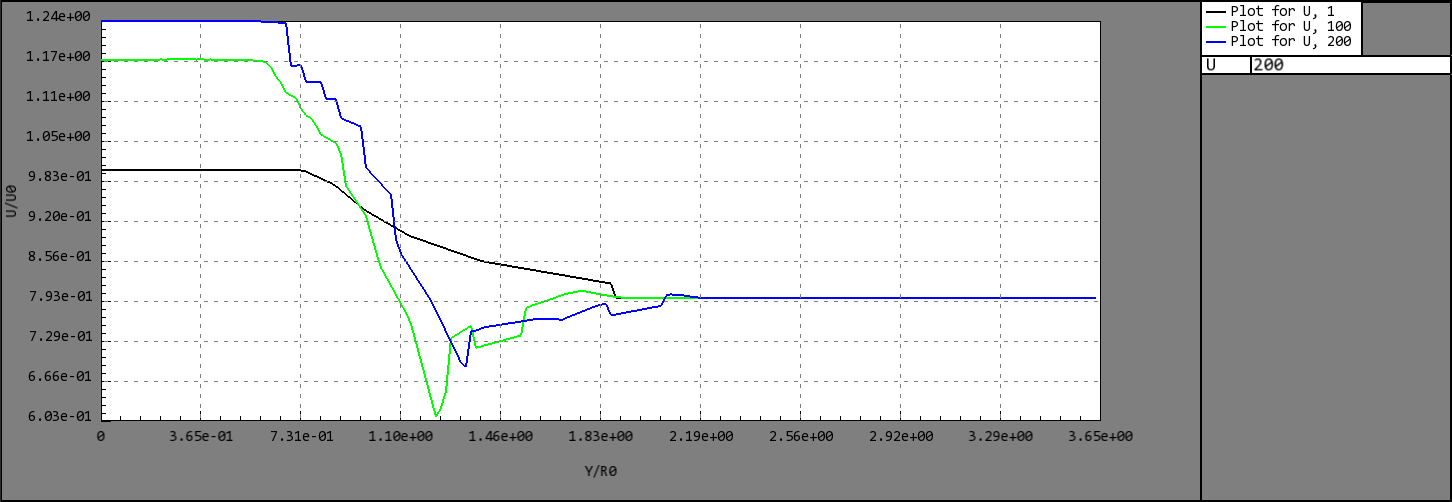
\includegraphics[width=15cm]{2-05-test2}
    \caption{Значение шага $0.0075$, параболизованная система}
    \label{fig:acc_2_1}
\end{figure}

\begin{figure}
    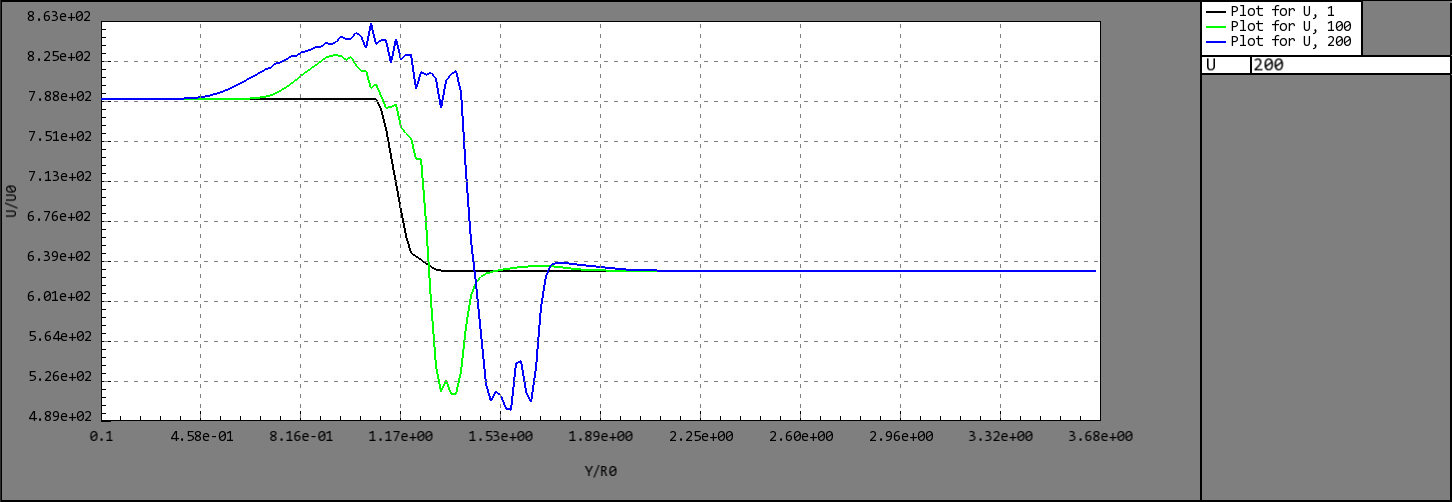
\includegraphics[width=15cm]{2-05-test5}
    \caption{Значение шага $0.0075$, полная система}
    \label{fig:acc_2_2}
\end{figure}

\begin{figure}
    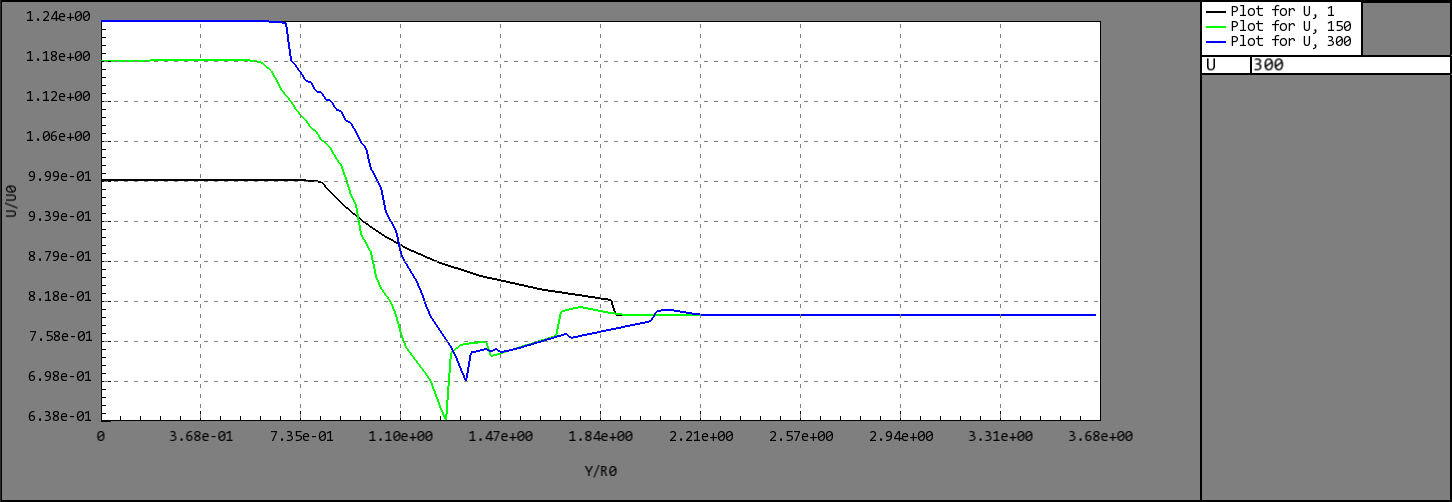
\includegraphics[width=15cm]{2-05-test3}
    \caption{Значение шага $0.0037$, параболизованная система}
    \label{fig:acc_3_1}
\end{figure}

\begin{figure}
    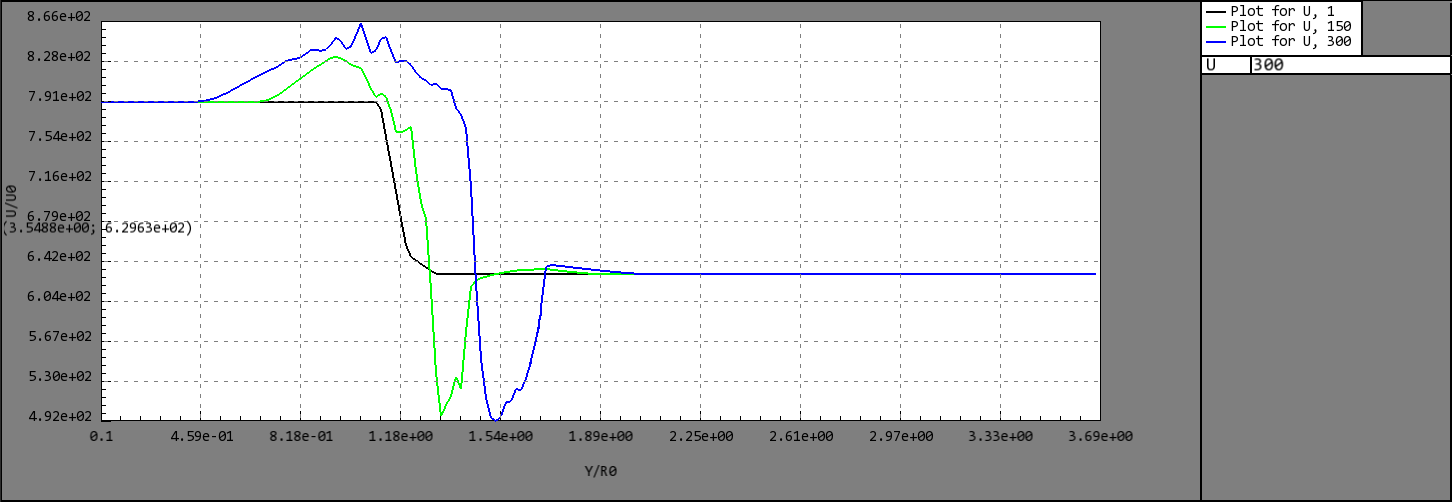
\includegraphics[width=15cm]{2-05-test6}
    \caption{Значение шага $0.0037$, полная система}
    \label{fig:acc_3_2}
\end{figure}

Наблюдаются две характерные области:

\begin{itemize}
\item При $H > 0.007L$ доминирует погрешность аппроксимации
\item При $H < 0.003$ основную роль играют ошибки округления
\end{itemize}

Оптимальным с точки зрения точности и вычислительных затрат оказался шаг $H \approx 0.003$.

\subsection{Сравнение полной и параболизированной систем уравнений}

Для оценки адекватности параболизированной постановки проведено сравнение с полной системой уравнений Навье-Стокса на тестовой задаче о турбулентной струе. Основные результаты представлены в таблице~\ref{tab:comparison}.

\begin{table}[h]
\centering
\caption{Сравнение характеристик течения для разных постановок}
\label{tab:comparison}
    \begin{tabular}{|l|c|c|}
    \hline
    Параметр & Полная система & Параболизированная \\ \hline
    Длина факела, м & 1.25 & 1.31 \\ 
    Макс. температура, K & 2150 & 2095 \\
    Время расчёта, с & 347.9 & 125.6 \\ \hline
    \end{tabular}
\end{table}

Наибольшие расхождения (до 12\%) наблюдаются в зоне обратных течений, где параболизированная постановка менее точна. Однако для основной зоны струи различия не превышают 5\%.

\subsection{Зависимость времени расчёта от шага дискретизации}
\label{subsec:performance}

Производительность алгоритма исследовалась на сетках различной плотности. Результаты представлены на рисунке~\ref{fig:performance}.

\begin{figure}
\centering
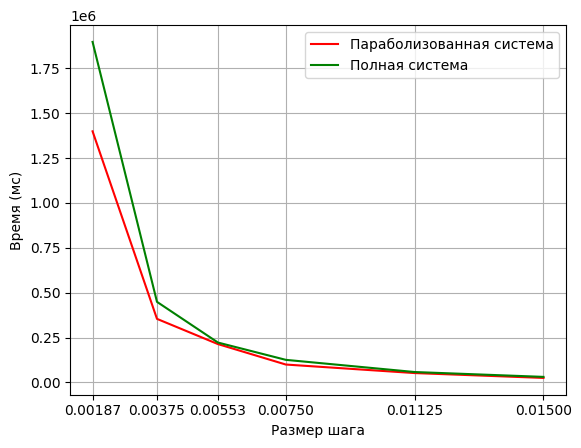
\includegraphics[width=0.8\linewidth]{2-05-time}
\caption{Зависимость времени расчёта от размера шага}
\label{fig:performance}
\end{figure}

Зависимость времени расчёта $T$ от размера шага $H$ хорошо аппроксимируется степенной функцией:
\begin{equation}
T(N) = aN^b
\end{equation}
где $b \approx 1.8$ для параболизированной и $b \approx 2.1$ для полной системы. Уменьшение показателя степени связано с эффективностью маршевого алгоритма.

\subsection{Прочие примеры}

Для демонстрации изменения различных переменных были выбраны следующие начальные данные и размеры шагов (Рис.~\ref{src:format}). Данный формат используется для всех тестовых случаев.

\begin{figure}
\begin{lstlisting}[language=Python, escapeinside=``]
    #R0
    0.01
    #конечный расчёт X - n*R_0
    100
    #конечный расчёт Y - n*R_0
    370
    #размер сетки
    200 500
    #размер профиля
    37
    #путь к базе данных для хим. кинетики
    ./../../test/ChemicTest/bufermm1.txt
    #значения внутри
    5
    U 790
    T 237
    P 50290
    MU 0.18e-4
    Y 1
    #количество переменных с ненулевым профилем
    6
    Y       U       V       W       T       P
    0.100   1.000   0.000   0.000   1.000   1.000
    0.200   1.000   0.000   0.000   1.000   1.000
    0.300   1.000   0.000   0.000   1.000   1.000
    0.400   1.000   0.000   0.000   1.000   1.000
    0.500   1.000   0.000   0.000   1.000   1.000
    0.600   1.000   0.000   0.000   1.000   1.000
    0.700   1.000   0.000   0.000   1.000   1.000
    0.800   1.000   0.000   0.000   1.000   1.000
    0.900   1.000   0.000   0.000   1.000   1.000
    1.000   1.000   0.000   0.000   1.000   0.455
\end{lstlisting}
\caption{Формат входных файлов}
\label{src:format}
\end{figure}

Результаты отображены на рисунках~\ref{fig:acc_U},\ref{fig:acc_V},\ref{fig:acc_MU},\ref{fig:acc_J},\ref{fig:acc_T},\ref{fig:acc_P},\ref{fig:acc_RHO}. Как можно заметить, даже при мелком шаге в расчётах присутствуют некоторые неточности и скачки. Это может быть вызвано неточной моделью турбулентности или издержками параболизации. В дальнейшем можно реализовать более точные модели и заняться более детальной оптимизацией.

\begin{figure}
    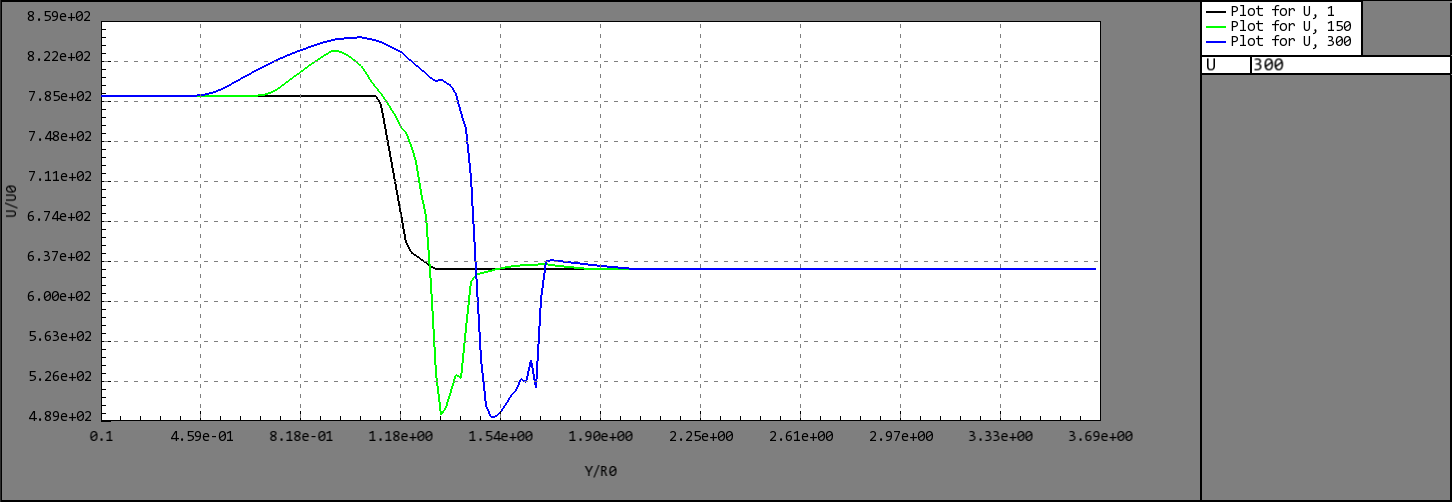
\includegraphics[width=15cm]{2-05-test-U}
    \caption{Значения скорости $U$}
    \label{fig:acc_U}
\end{figure}

\begin{figure}
    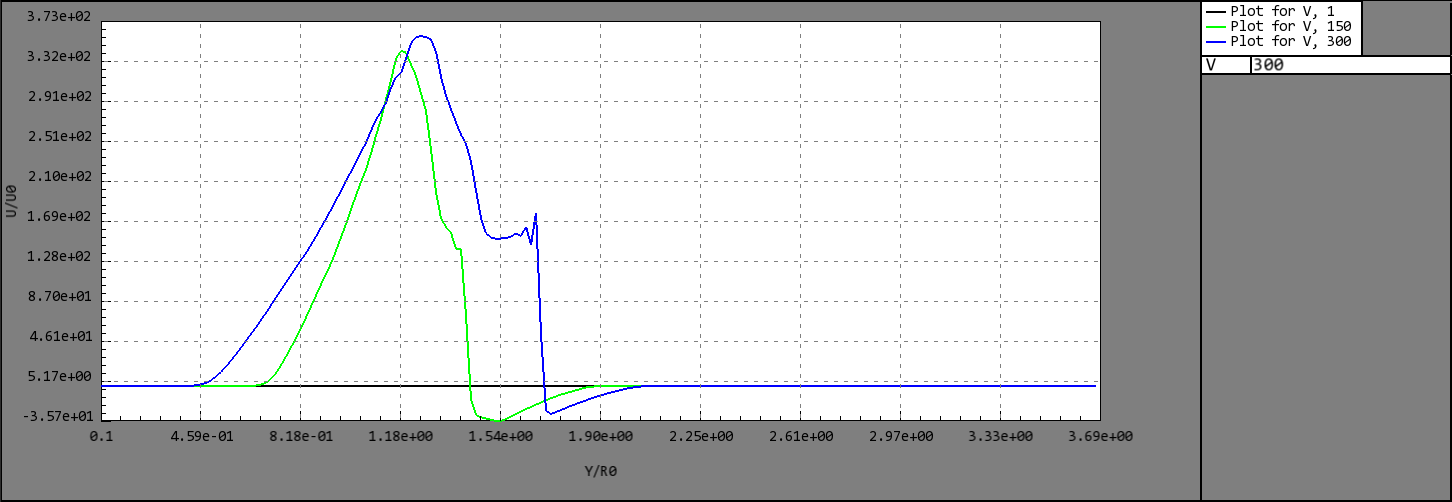
\includegraphics[width=15cm]{2-05-test-V}
    \caption{Значения скорости $V$}
    \label{fig:acc_V}
\end{figure}

\begin{figure}
    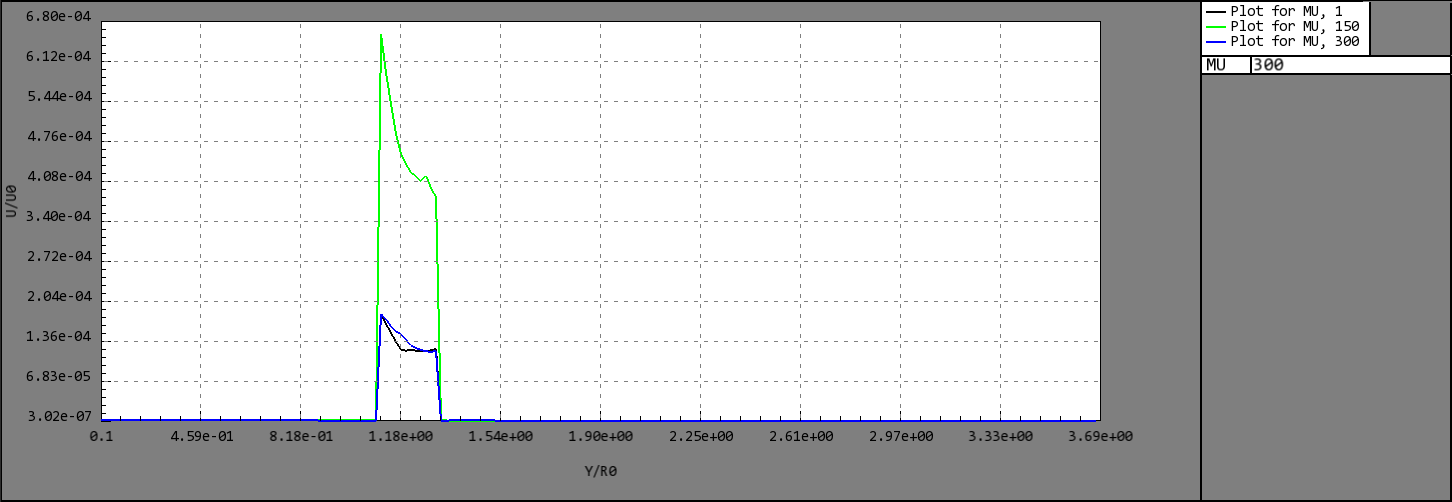
\includegraphics[width=15cm]{2-05-test-MU}
    \caption{Значения вязкости $\mu$}
    \label{fig:acc_MU}
\end{figure}

\begin{figure}
    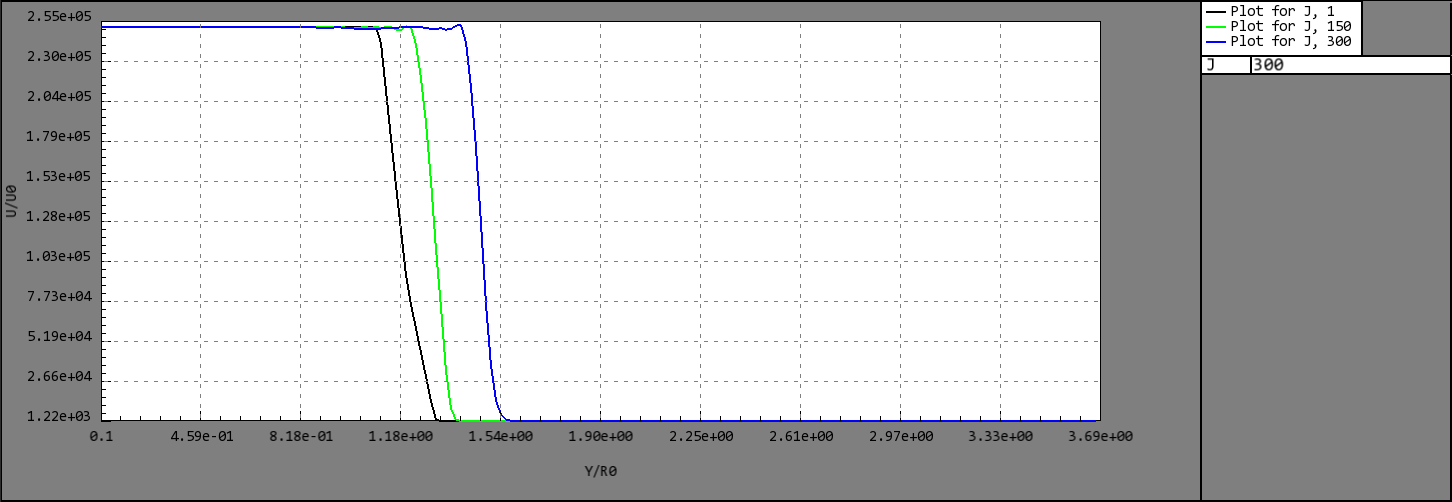
\includegraphics[width=15cm]{2-05-test-J}
    \caption{Значения энтальпии $J$}
    \label{fig:acc_J}
\end{figure}

\begin{figure}
    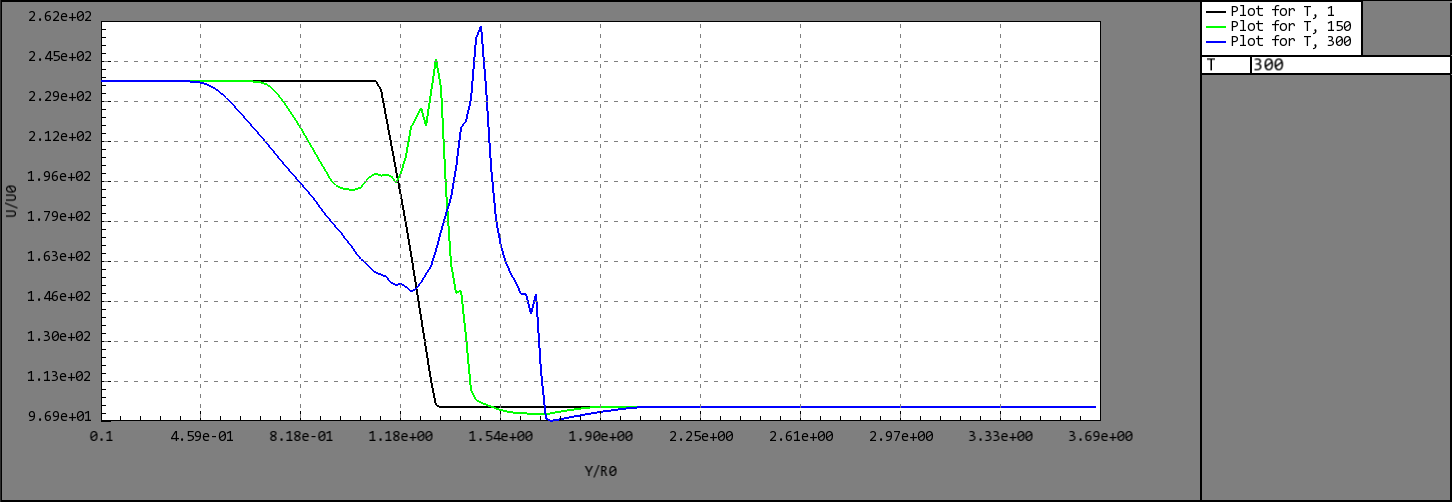
\includegraphics[width=15cm]{2-05-test-T}
    \caption{Значения температуры $T$}
    \label{fig:acc_T}
\end{figure}

\begin{figure}
    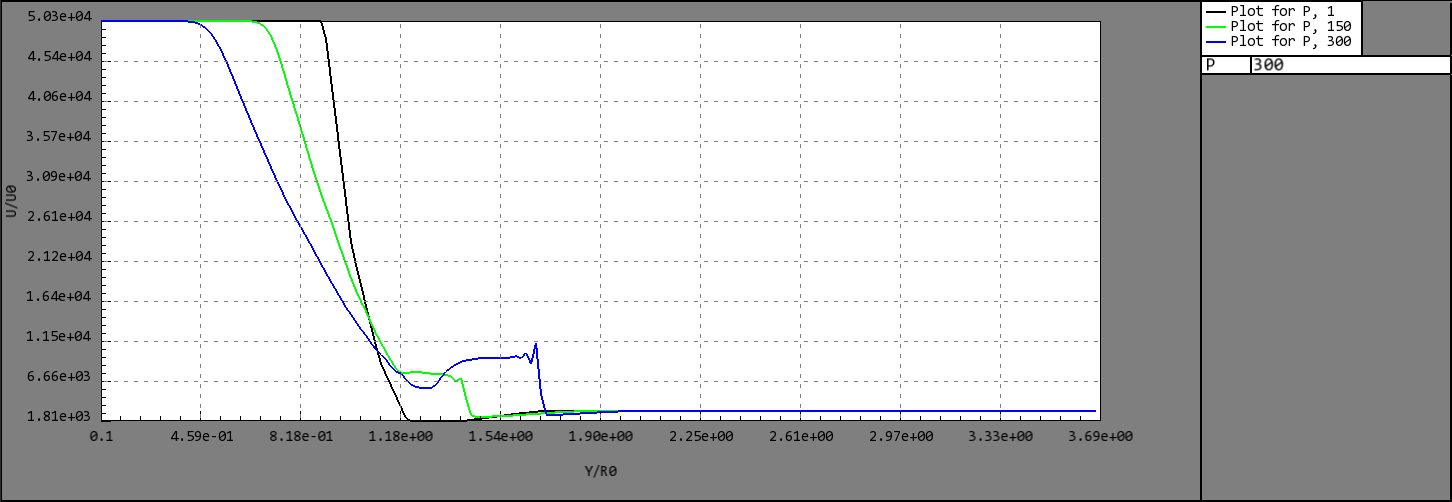
\includegraphics[width=15cm]{2-05-test-P}
    \caption{Значения давления $P$}
    \label{fig:acc_P}
\end{figure}

\begin{figure}
    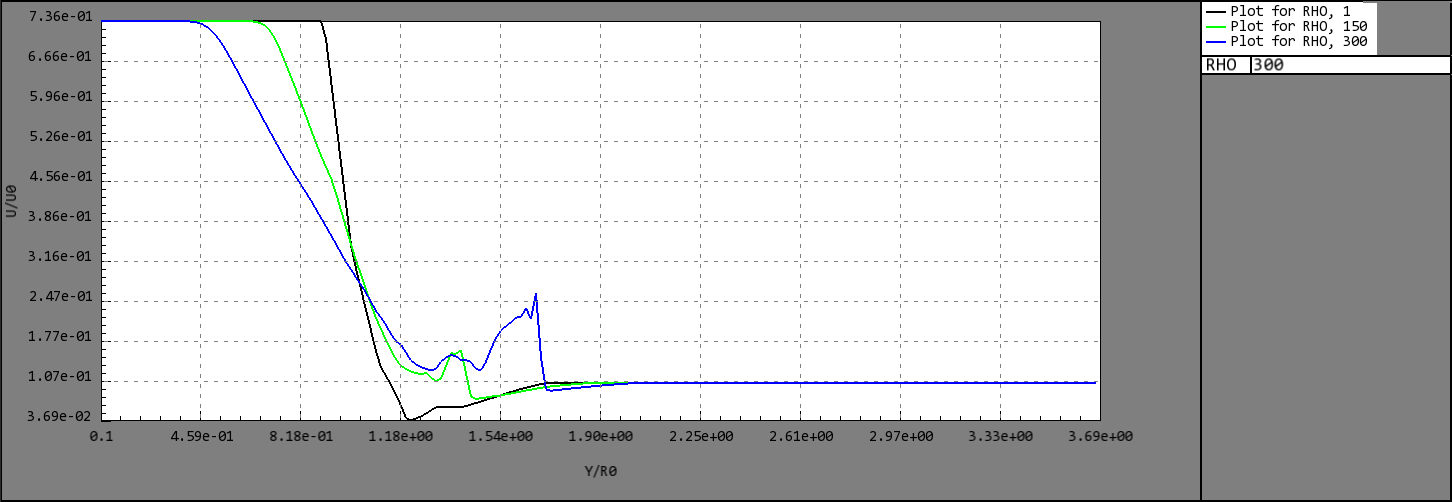
\includegraphics[width=15cm]{2-05-test-RHO}
    \caption{Значения плотности $\rho$}
    \label{fig:acc_RHO}
\end{figure}

Проведенные тесты показали:
\begin{itemize}
\item Параболизированная постановка обеспечивает разумный компромисс между точностью и производительностью
\item Оптимальный шаг дискретизации составляет $\Delta x \approx 0.03L$
\item Время расчёта растет почти квадратично с увеличением числа узлов (уменьшением шага)
\end{itemize}